\subsection{Matching}

Unter Matching eines Graphen versteht man eine Menge von Kanten von G, sodass keine zwei Kanten einen Knoten gemeinsam haben.

\begin{figure}[h]
\centering
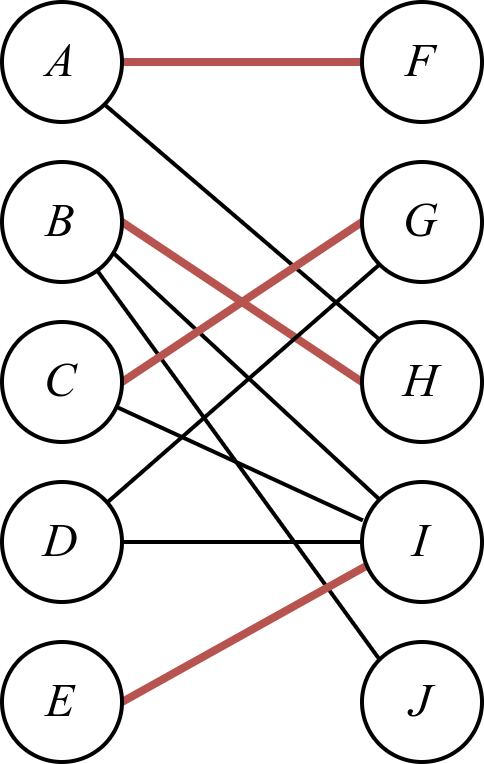
\includegraphics[width=0.2\textwidth]{graphics/graph_matching.png}
\end{figure}

$M = {(A,F), (B,H), (C,G), (E,I)}$ ist ein Matching der Mächtigkeit 4

\subsubsection*{Heiratssatz}

Im bipartiten Graphen $G = (S + T, E)$ gilt:

$$
m(G) = |S| \Leftrightarrow |A| \leq |N (A)| \text{ für alle } A \subseteq S
$$

\subsubsection*{Hopcraft-Karp Algorithmus}

